\subsection{Theory}

\begin{frame}{Utilities for the parareal method}
	
	\small
	What is the parareal method ?
	\begin{enumerate}[\textbullet]
		\item parallel-in-time integration method, introduced in 2001 by Lions, Maday and Turinici\footnote[frame]{\url{https://en.wikipedia.org/w/index.php?title=Parareal&oldid=1047894968}}
		\item computes the numerical solution for multiple time steps in parallel
		\item categorized as a parallel-across-the-steps method 
	\end{enumerate}

	Time decomposition :
	\begin{enumerate}[\textbullet]
		\item $[t_0,T]=[t_0,t_1]\cup\dots\cup[t_{P-1},t_P]$ with $t_P=T$ and $P=$number of processes
	\end{enumerate}

	\begin{minipage}{.68\linewidth}
		Notation :
		\begin{enumerate}[\textbullet]
			\item $F$ : high accuracy integrator, \quad $\Delta t_F$ : time step \\
			$G$ : low accuracy integrator, \quad $\Delta t_G$ : coarse time step
			\item $U_j^k, j\in\{0,\dots,P\}$ : initial point at time $t_j$ and at iteration $k$.
		\end{enumerate}
	\end{minipage}
	\begin{minipage}{.28\linewidth}
		\qquad 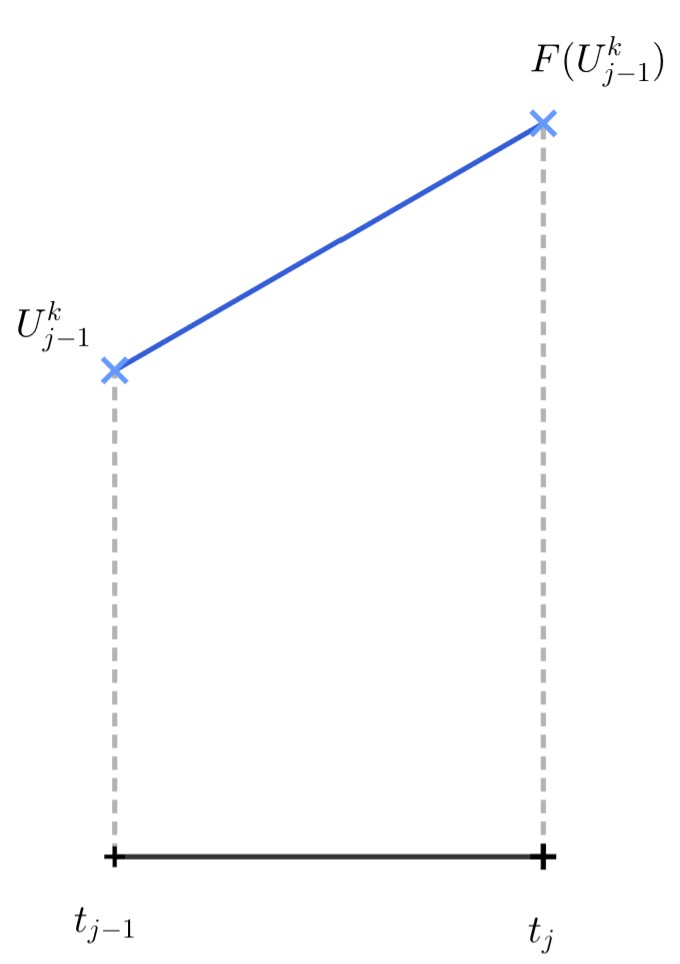
\includegraphics[width=0.7\linewidth]{images/parareal/explane_F.jpg}
	\end{minipage}
	\begin{enumerate}[\textbullet]
		\item $F(U_{j-1}^k), j\in\{1,\dots,P\}$ : value of the fine integrator at $t_j$ starting by $U_{j-1}^k$ (resp. $G(U_{j-1}^k)$)
	\end{enumerate}
	
\end{frame}

\begin{frame}[allowframebreaks]{Explanation of the parareal method}
	\begin{figure}
		\centering
		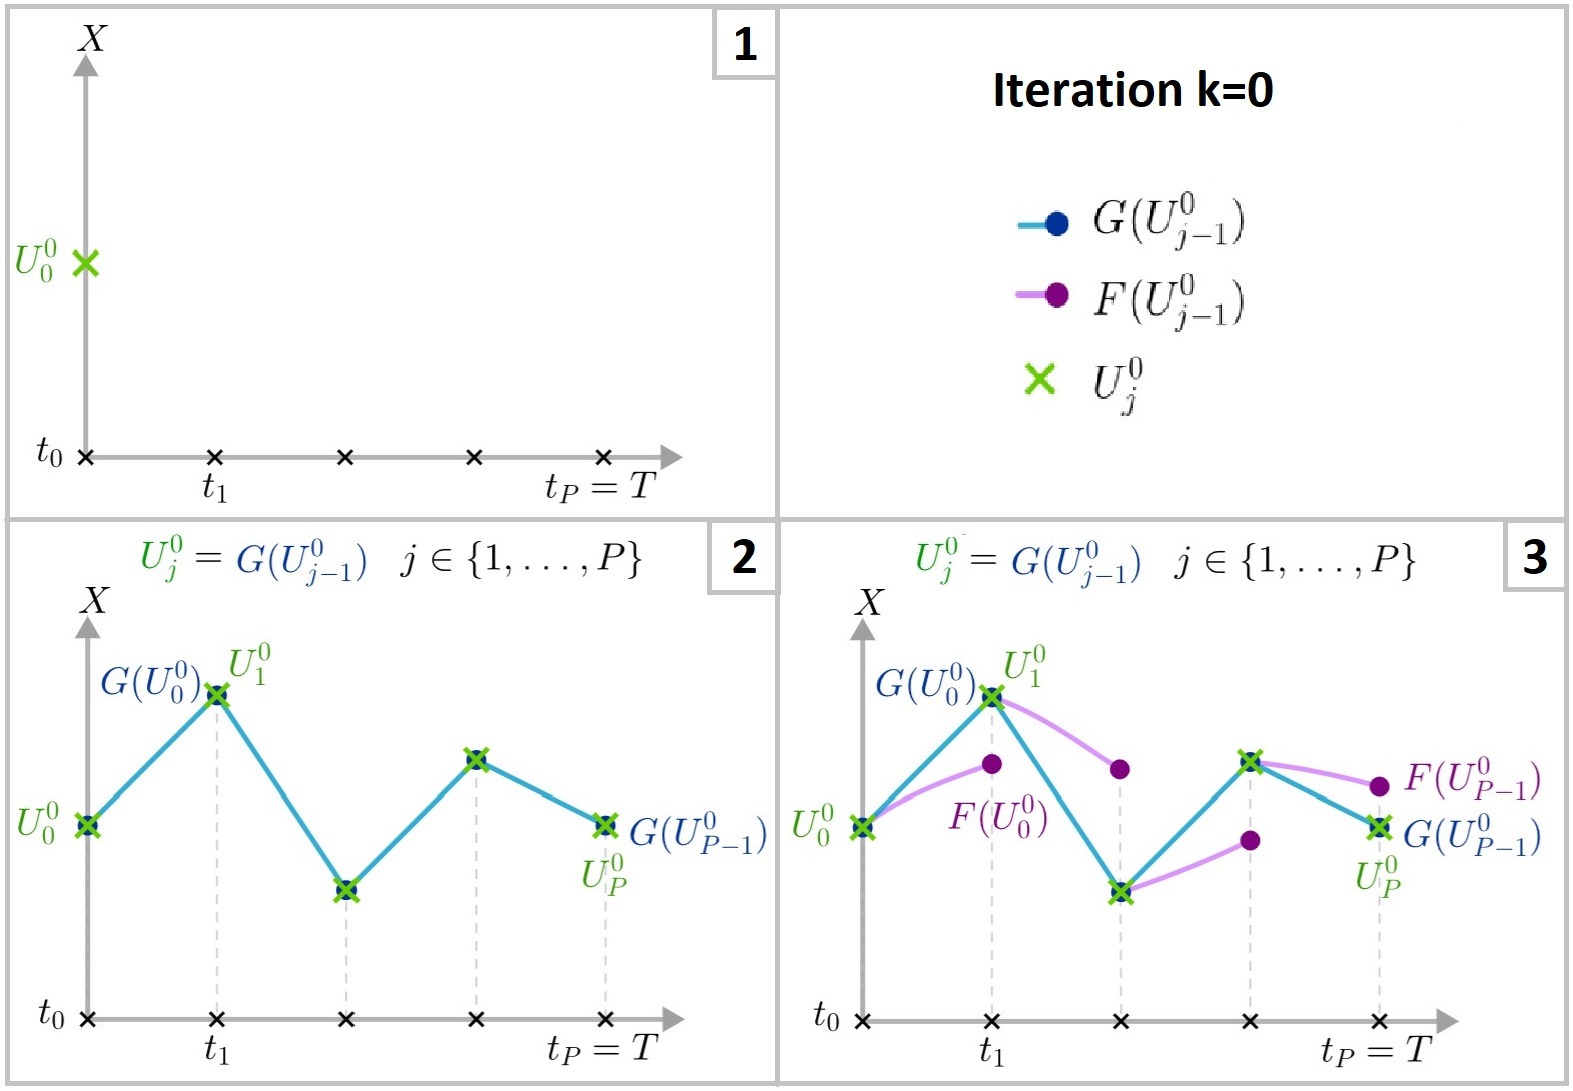
\includegraphics[width=0.6\linewidth]{images/parareal/parareal_k0.jpg}
	\end{figure}
	\begin{figure}
		\centering
		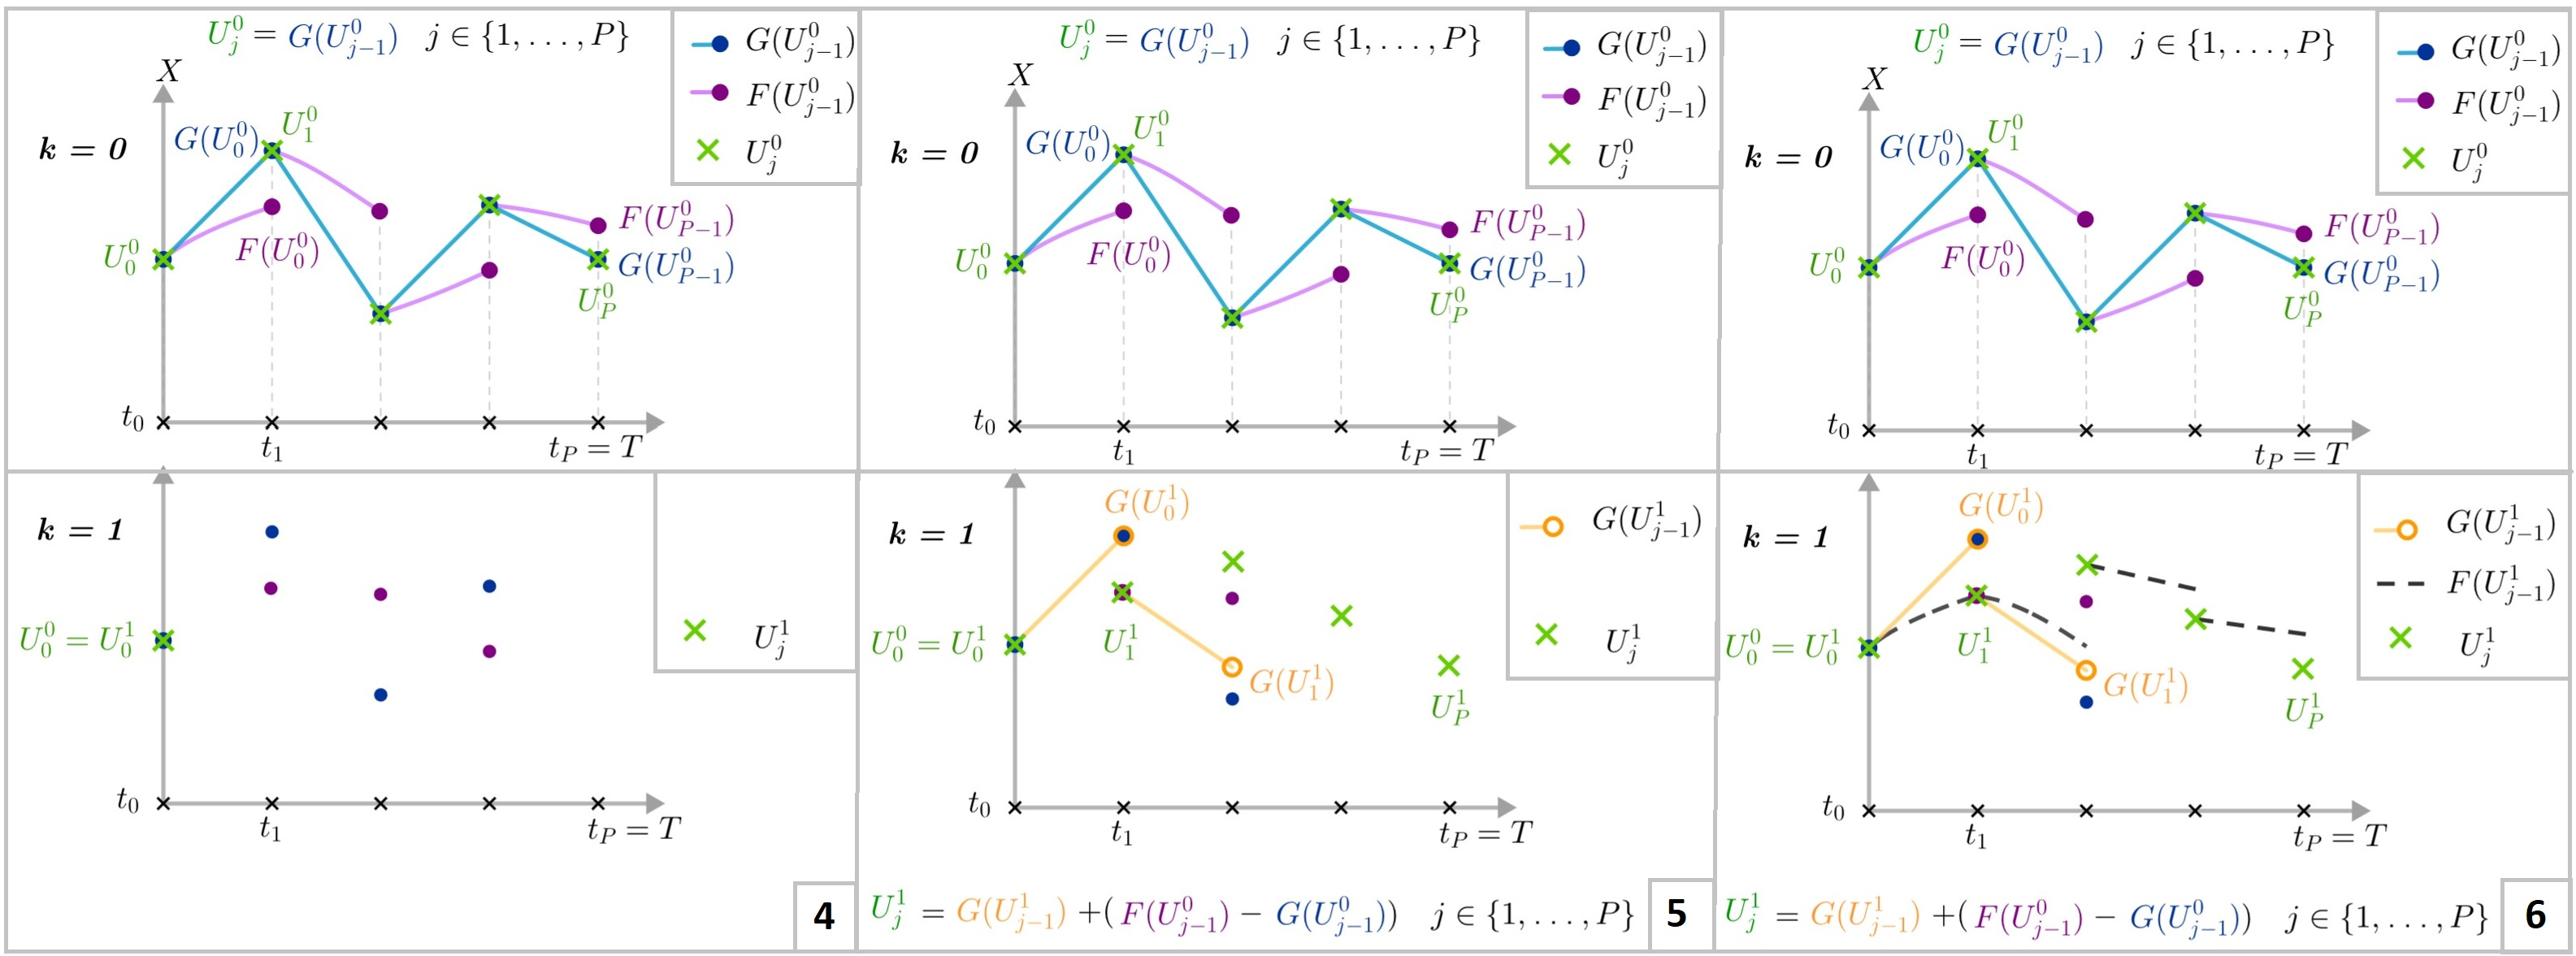
\includegraphics[width=\linewidth]{images/parareal/parareal_k1.jpg}
	\end{figure}
	\small
	We have at iteration $k$ :
	$$U_j^k=G(U_{j-1}^k)+(F(U_{j-1}^{k-1})-G(U_{j-1}^{k-1}))$$
\end{frame}

\begin{frame}{Order of the method}
	The parareal method is of order k if there is a constant $c_k$ such that :
	\begin{equation*}
		\forall j\in\{0,\dots,P-1\} \qquad \mathcal{E}(j,k)\le c_k(\Delta t_G)^k
	\end{equation*}
	with
	$$\mathcal{E}(j,k)=|U_j^k-U_{ex}(t_j)|+\max_{t\in[t_j,t_{j+1}]}|U_k(t)-U_{ex}(t)|$$
	where 
	\begin{enumerate}[\textbullet]
		\item $U_j^k$ : initial point at $t_j$ and iteration $k$
		\item $U_{ex}(t_j)$ : exact solution at $t_j$ and iteration $k$
		\item $U_k$ : solution between $t_0$ and $T$ at iteration k
		\item $U_{ex}$ : exact solution between $t_0$ and $T$
	\end{enumerate}
	Note that we calculate the maximum just between $t_j$ and $t_{j+1}$.
\end{frame}

\subsection{Results}

\begin{frame}[allowframebreaks]{Harmonic oscillator}
	Equation :
	\begin{equation*}
		\frac{\partial^2 x}{\partial t^2}+\omega_0^2 x = 0 \quad \text{with} \quad \omega_0=\sqrt{\frac{k}{m}}.
		\label{osc}
	\end{equation*}
	
	Exact solution :
	$$x(t) = x_0 \cos(\omega_{0}t+\phi_0).$$ 
	
	\; \\
	
	2nd order differential equation $\rightarrow$ system of two first order equations :
		
	$$\qquad \frac{\partial x}{\partial t}=v \quad \Rightarrow \quad \left\{\;\begin{aligned}
		\frac{\partial x}{\partial t}&=v \\
		\frac{\partial v}{\partial t}&=-\omega_0^2 x
	\end{aligned}\right.
	$$  
	
	\newpage
	
	$$P=3, \quad x(0)=0,\quad v(0)=1, \quad\omega_0=5, \quad x_0=\frac{-1}{5}, \quad \phi_0=\frac{\pi}{2}$$
	\begin{minipage}{0.6\linewidth}
		\centering
		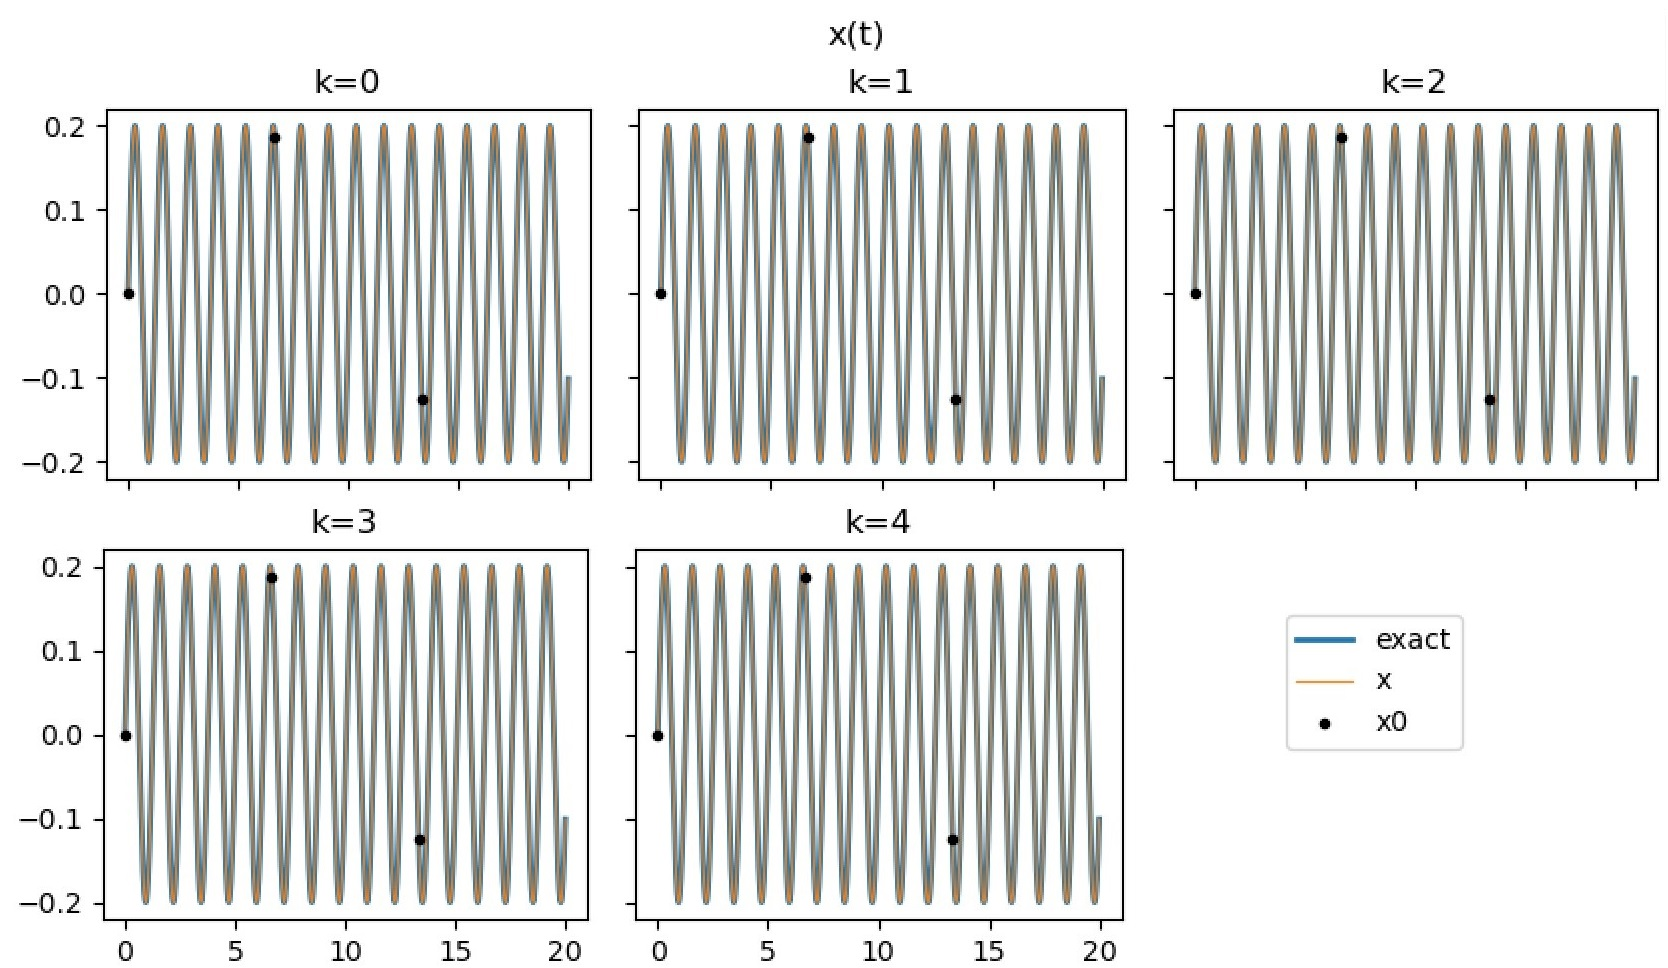
\includegraphics[width=\linewidth]{"images/parareal/osci_1.jpg"}
	\end{minipage} \;
	\begin{minipage}{0.38\linewidth}
		\centering
		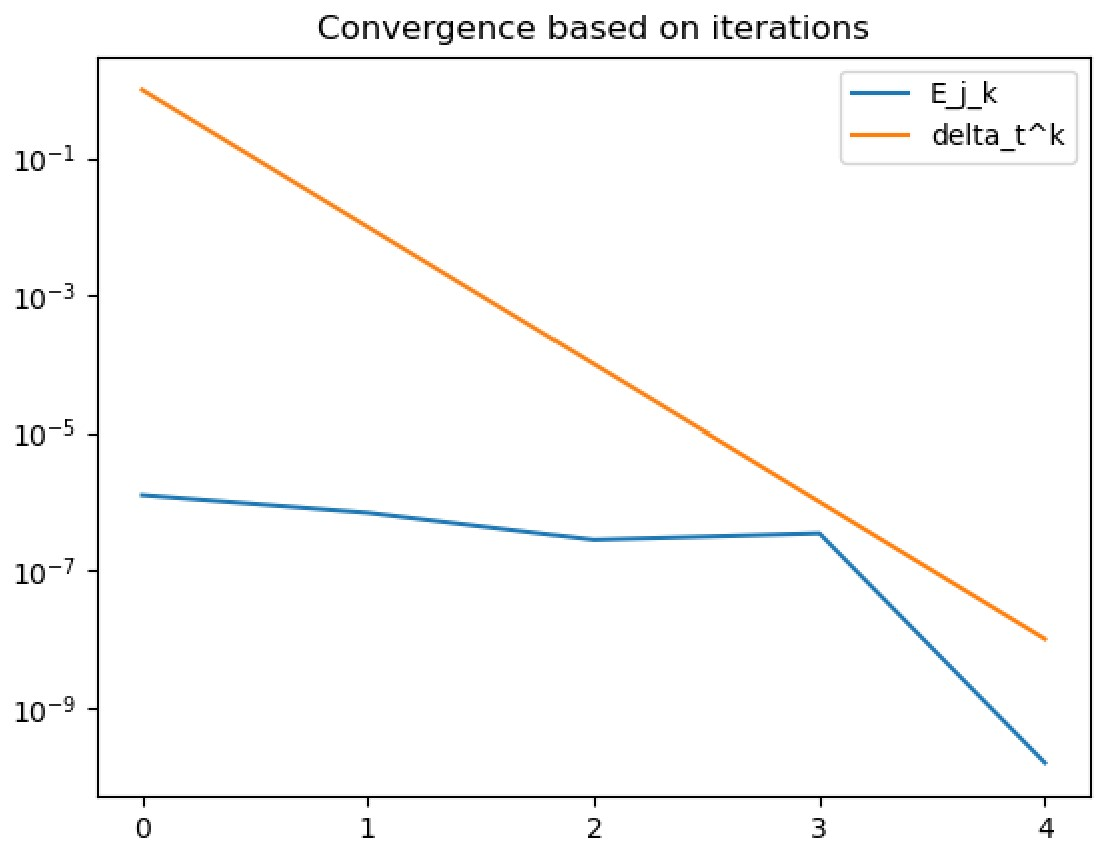
\includegraphics[width=\linewidth]{"images/parareal/osci_cvg_1.jpg"}
	\end{minipage}
	
\end{frame}

\begin{frame}[allowframebreaks]{Lorenz system}
	\begin{minipage}{\linewidth}
		\centering
		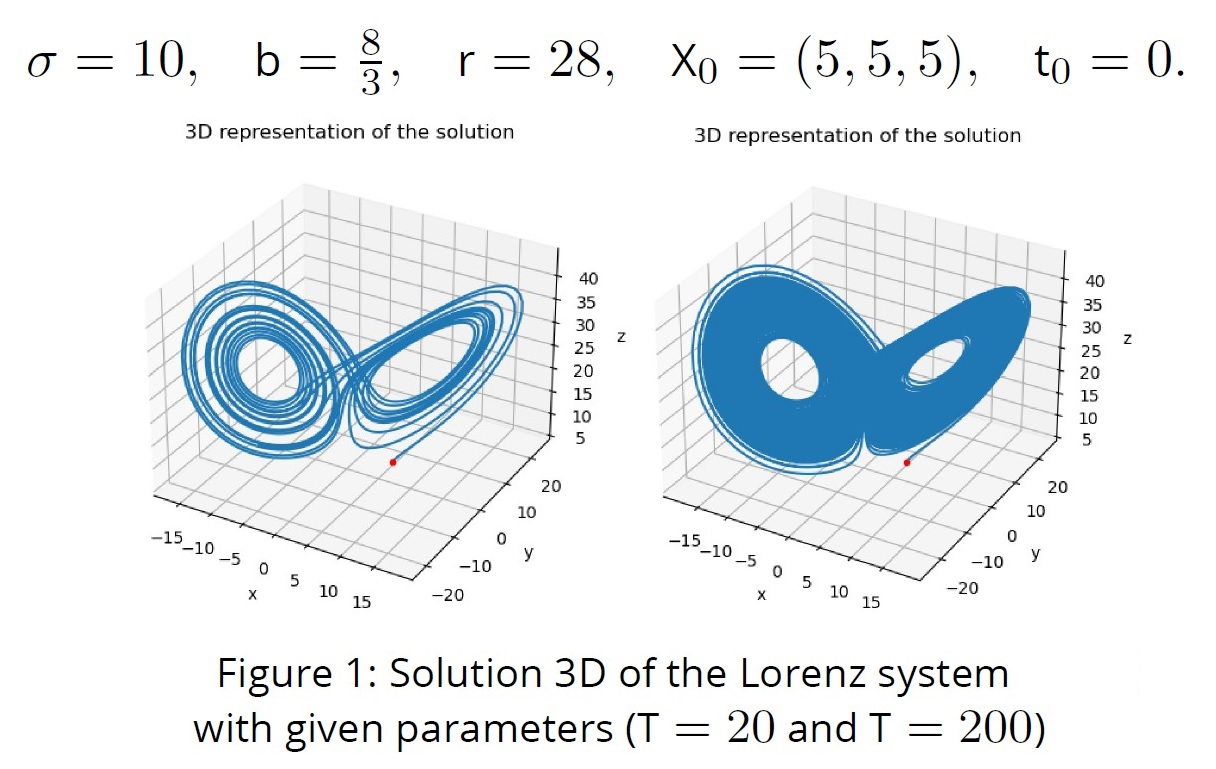
\includegraphics[width=0.8\linewidth]{"images/parareal/lorenz_sol3D.jpg"}
	\end{minipage}

	\newpage

	\begin{minipage}{\linewidth}
	\begin{figure} 
		\centering     
		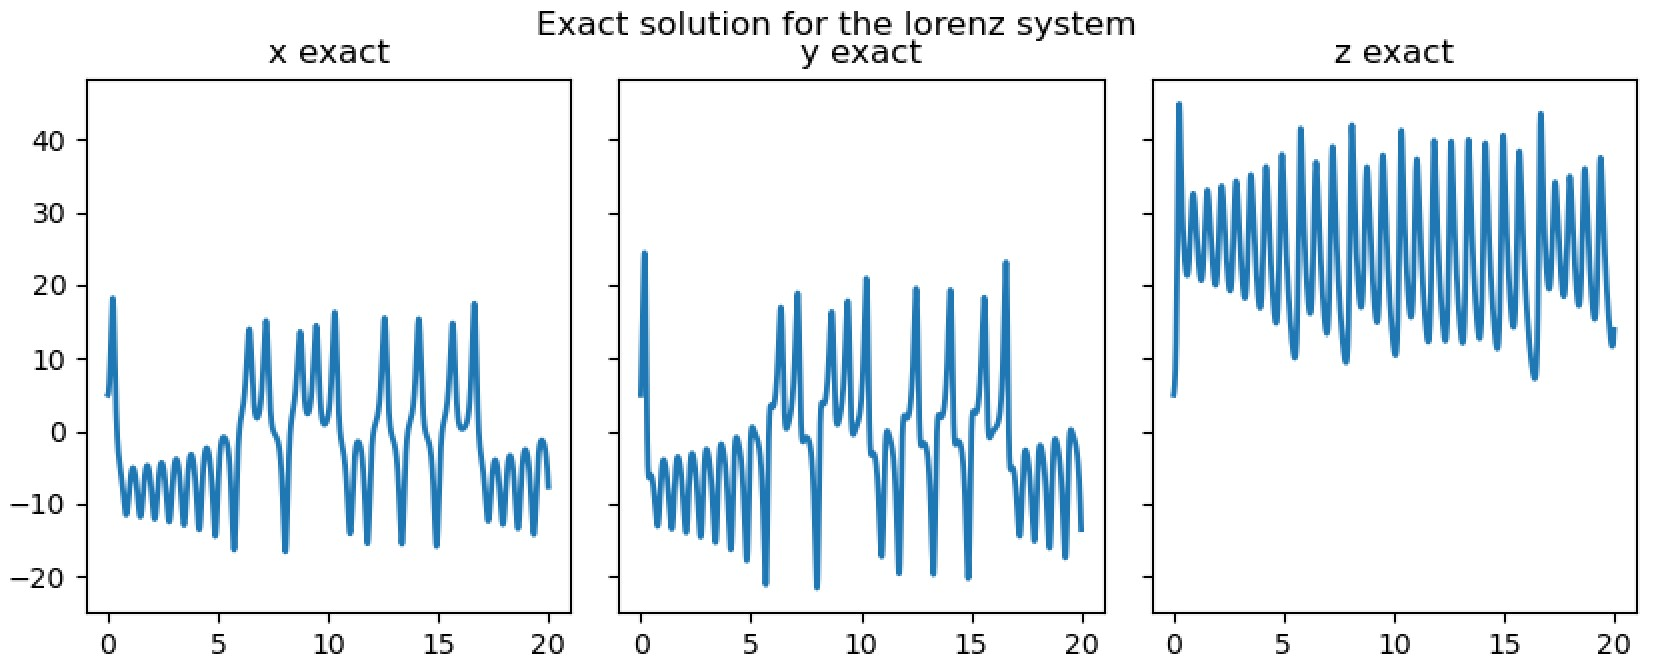
\includegraphics[width=\linewidth]{"images/parareal/lorenz_exact.jpg"}
		\caption{Solution of the Lorenz system with given parameters}
	\end{figure}
	\end{minipage}

	\newpage
	
	\begin{minipage}{\linewidth}
	\begin{figure}
		\centering       
		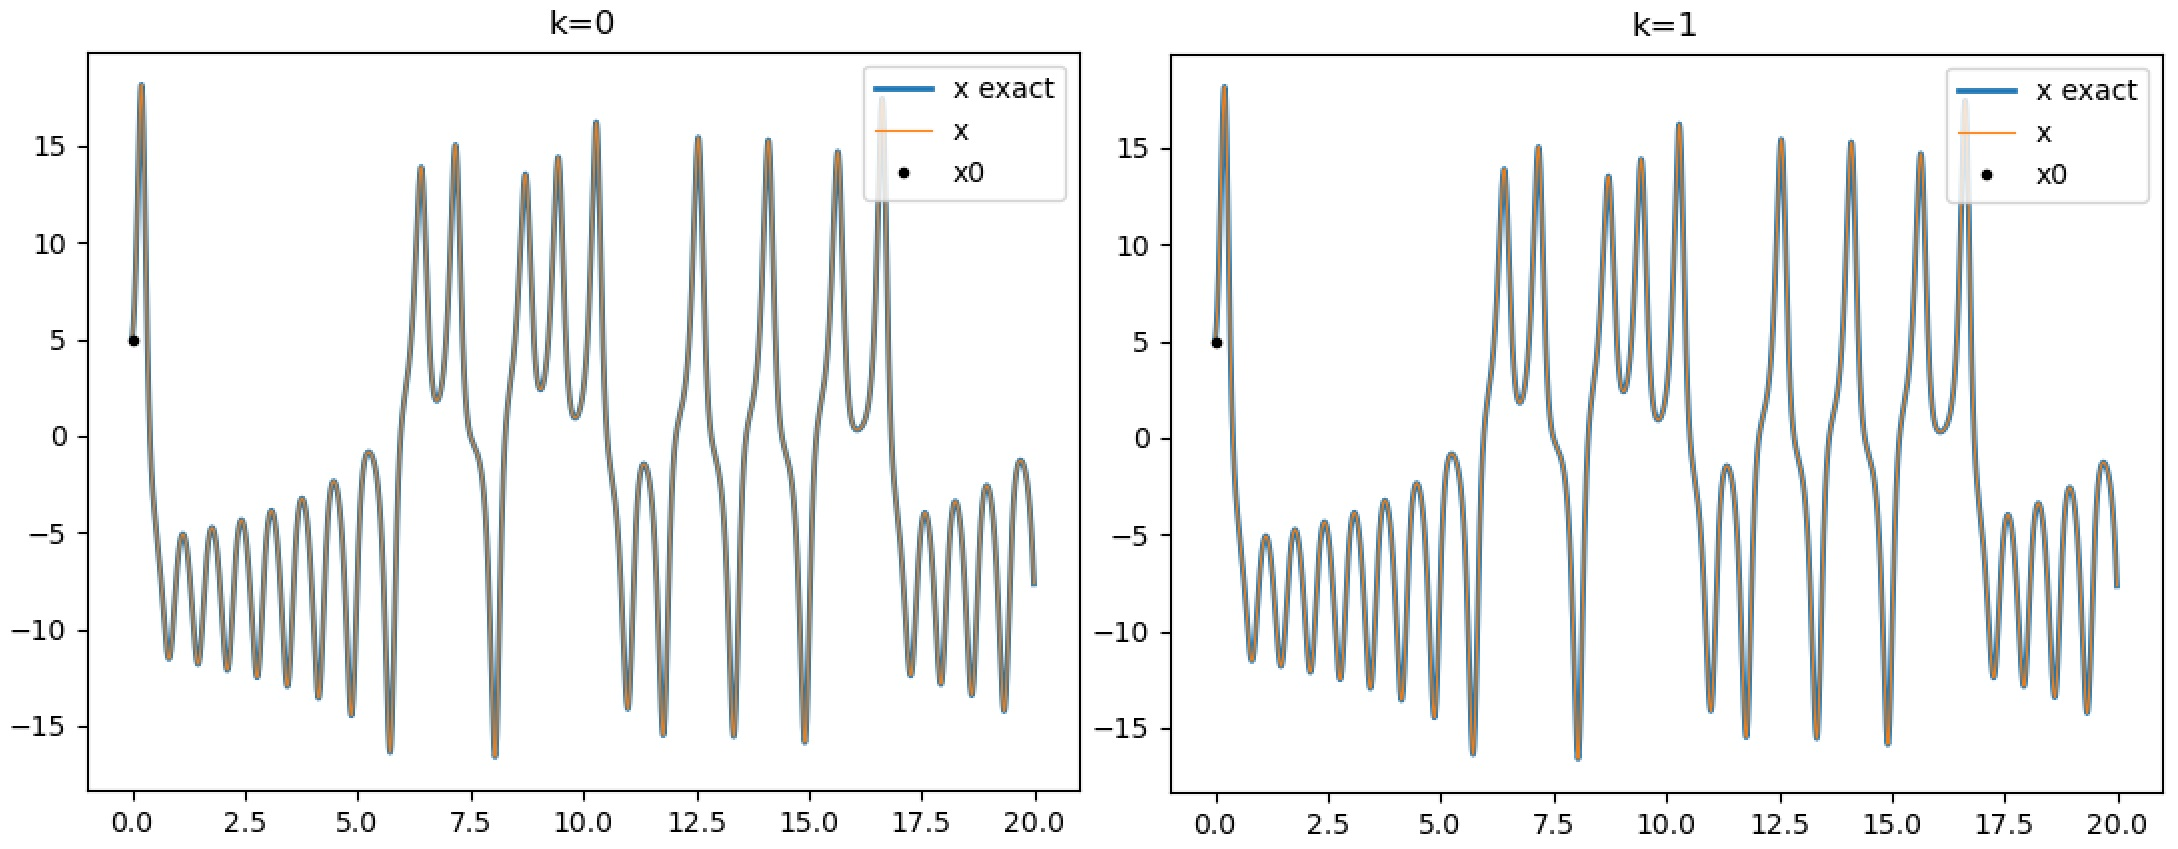
\includegraphics[width=0.9\linewidth]{"images/parareal/lorenz_1p.jpg"}
		\caption{Parareal method on the Lorenz system with 1 process}
	\end{figure}
	\end{minipage}

	\newpage

	\begin{minipage}{\linewidth}
	\begin{figure}
		\centering       
		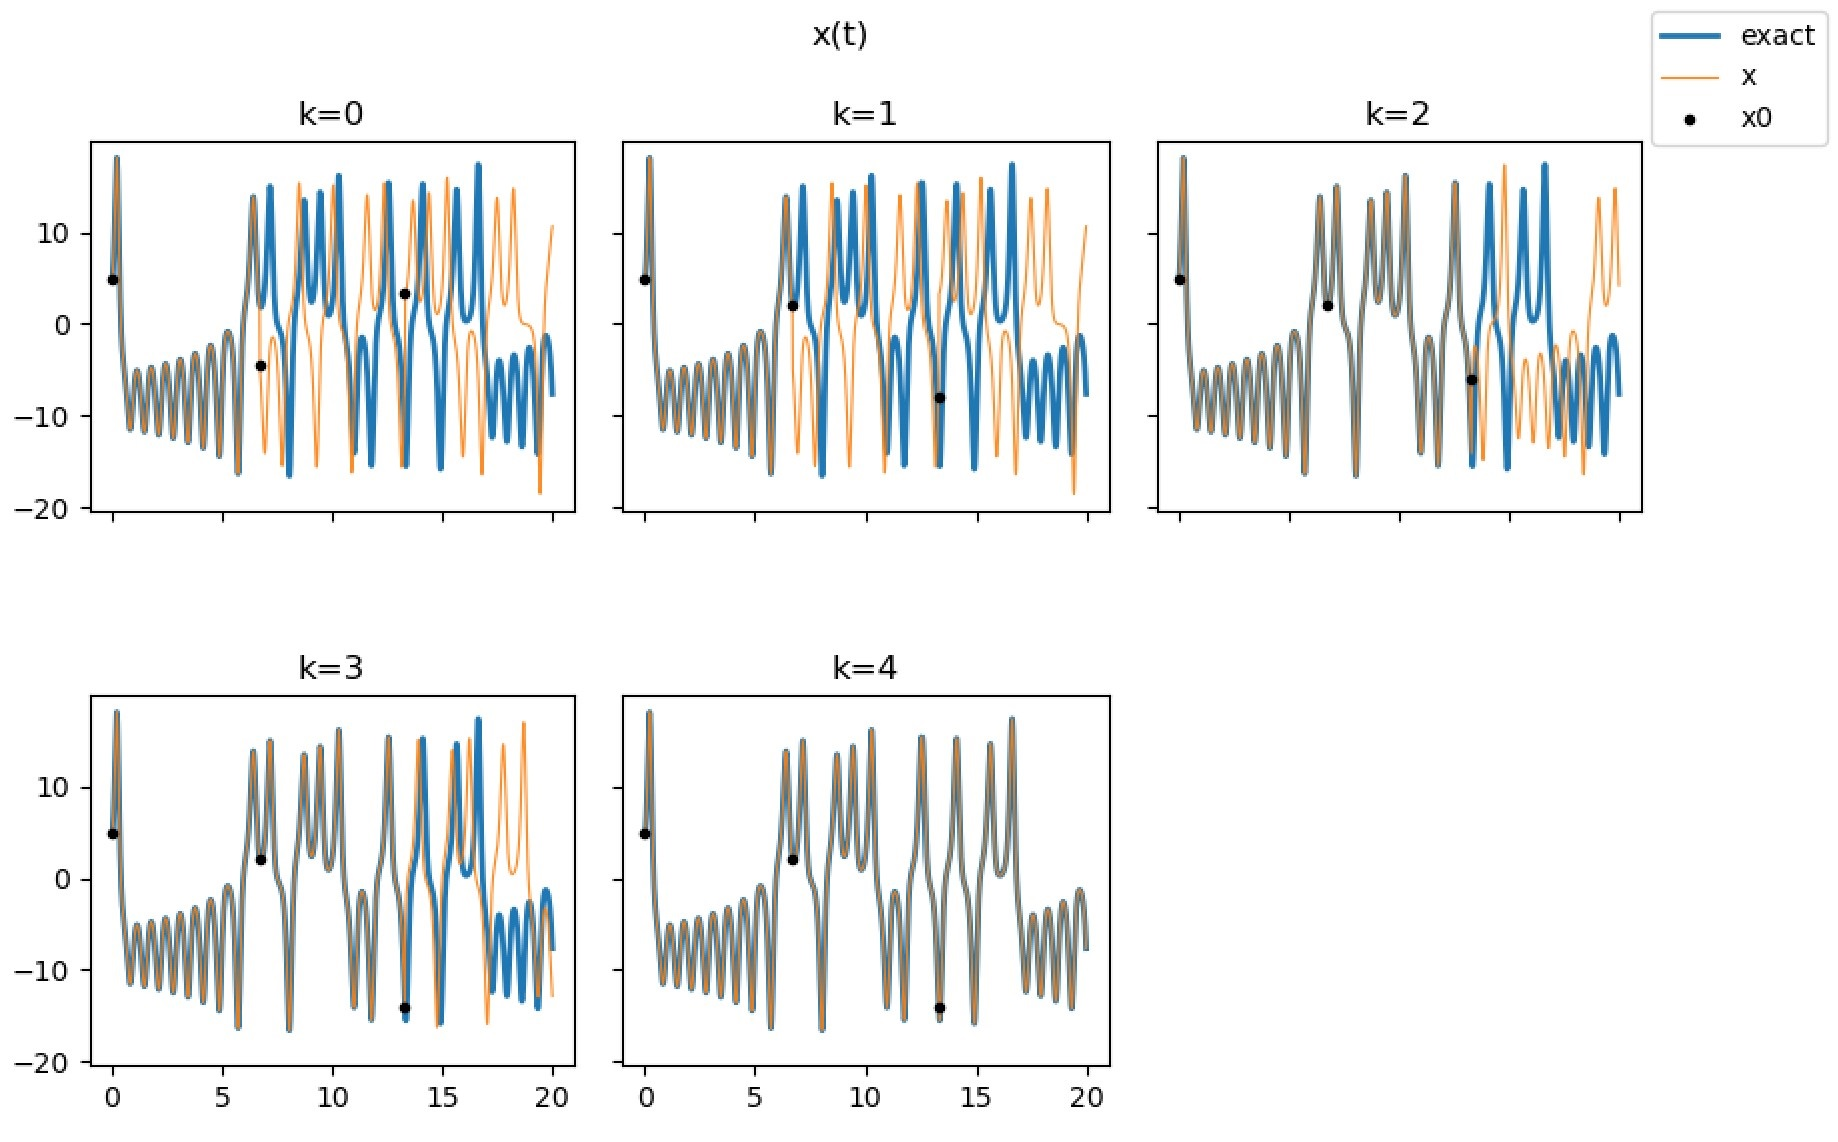
\includegraphics[width=0.7\linewidth]{"images/parareal/lorenz_3p.jpg"}
		\caption{Parareal method on the Lorenz system with 3 processes}
	\end{figure}
	\end{minipage}

	
	\begin{table}[H]
		\centering
		\begin{tabular}{| c || c | c | c | c | c |}
			\hline
			\multirow{2}{1.5 cm}{$\Delta t$} & \multirow{2}{1.5 cm}{Seq} & \multirow{2}{1.5 cm}{1 proc} & \multirow{2}{1.5 cm}{2 proc} & \multirow{2}{1.5 cm}{3 proc} &\multirow{2}{1.5 cm}{4 proc} \\
			& & & & & \\
			\hline 
			F : 0.0025 & \multirow{2}{1.5 cm}{30s} & \multirow{2}{1.5 cm}{36s} & \multirow{2}{1.5 cm}{10s} & \multirow{2}{1.5 cm}{9,7s} & \multirow{2}{1.5 cm}{9,4s} \\
			G : 0.025 & & & & & \\
			\hline 
			F : 0.00125 & \multirow{2}{1.5 cm}{1m19} & \multirow{2}{1.5 cm}{1m42} & \multirow{2}{1.5 cm}{39s} & \multirow{2}{1.5 cm}{32s} & \multirow{2}{1.5 cm}{29s} \\
			G : 0.0125 & & & & & \\
			\hline 
			F : 0.001 & \multirow{2}{1.5 cm}{1m52} & \multirow{2}{1.5 cm}{3m40} & \multirow{2}{1.5 cm}{1m56} & \multirow{2}{1.5 cm}{1m29} & \multirow{2}{1.5 cm}{1m16} \\
			G : 0.01 & & & & & \\	 
			\hline
		\end{tabular}
		\caption{Execution time for various time steps ($T=200$).}
		\label{time}
	\end{table}

\end{frame}